\documentclass[a4paper]{article}

\usepackage{fullpage} % Package to use full page
\usepackage{parskip} % Package to tweak paragraph skipping
\usepackage{tikz} % Package for drawing
\usepackage{amsmath}
\usepackage{hyperref}
\usepackage{enumitem}
\usepackage[bottom]{footmisc}
\usepackage{caption}
\usepackage{subcaption}


\title{Modeling the dynamics of an institutionalized leading class in the context of collective action}
\author{Claire Gu\'{e}rin}
\date{\today}

\begin{document}

\maketitle

\section{Life cycle}
\label{sec:lifcyc}

I model the structural evolution of an initially non-complex (unstratified) human society. The population is constituted of N producers, who extract resources from the territory pertaining to the social group. An instance would be agriculturalist societies that grow food crops and rear animals for farming. Adults gather to solve collective action problems in order to improve extraction efficiency in the following generation (medium-term effect). Such actions would be typically exemplified by the construction of an irrigation system that would improve harvest yield for every producer. 

During childhood, individuals in the population acquire two vertically transmissible cultural traits that are respectively expressed as two distinct social behaviors:

\begin{enumerate}
	\item personal investment into a public good dedicated to the functioning of a common institution;
	\item personal preference for the modalities of public good allocation.
\end{enumerate} 

Individuals are attributed a lifetime temporal budget, which constrains a trade-off of time investment in different activities:

\begin{itemize}
	\item extracting resources
	\item solving collective action problems
\end{itemize}
	
Adults invest part of their own extracted resources into the public good, proportional to their social involvement (first behavioral trait). 
Upon reach of adulthood, some individuals can be elected as leaders who are delegated to invest more time into solving collective action problems of their generation. The collective action problem specifically consists in reaching a consensus over deciding the proportions of public good that will be allocated to resources extraction efficiency and detection and sanctioning of cheaters respectively. Cheaters are individuals who exploit the system by benefiting from productivity enhancement, while investing few the public good.  

The individual trait that determines budget allocation preferences is secondarily influenced by the preference of same-generation peers, which is differentially conveyed through social network and with success dependent on reputation. Hence, leaders have more chances of influencing individual preferences for public budget allocation. To compensate for their time budget sacrifice (resulting in a decreased resources extraction), leaders are entitled to ask for a portion the resources produced by non-leaders, in the form of taxes.

Upon reach of consensus based on a time-dependent aggregation rule, individuals reproduce differentially as their lifetime reproductive success depends on their final resources. Reproduction is clonal, with non-overlapping generations characterized by discrete time.     

\section{Social class dynamics}
\label{sec:elec}

Let the population size at time $t$ be $N^t$. At every generation, a proportion $\lambda$ of individuals are elected in order to take on the role of political leaders in institution decisions. I use the term election in a broad sense, as leaders can be chosen explicitly through official vote or implicitly as tacit agreement among social members of the population \footnote{What determines an individual's probability to be elected? Do they bear an intrinsic quality that renders them more suitable for leadership? cf Tsimane': body size, social connections, generosity, etc.}. 
In this model, leaders are randomly drawn from the population at each generation \footnote{Heritability of leadership = greater probability to be elected if parent was leader (nepotism)?}.
The total population size $N^t$ amounts to the number of leaders and producers at time $t$, $n_L^t$ and $n_P^t$ respectively. At the next generation, I have:

\begin{equation}
	\begin{cases}
	n_L^{t+1}=\lambda\left[n_L^t\cdot w(n_L^t)+n_P^t\cdot w(n_P^t)\right]\\
	n_P^{t+1}=(1-\lambda)\left[n_L^t\cdot w(n_L^t)+n_P^t\cdot w(n_P^t)\right]
	\end{cases}
\end{equation}

Were $w$ corresponds to fitness estimated by lifetime reproductive success. $\lambda$ is not constant but a variable that changes over time. Indeed, I assume that the proportion of leaders in the population are an informed choice from the people based on leadership efficiency in the direct previous generation (parental, fig. \ref{fig:lambda}) \footnote{NB: Function parameters if the figure obviously need to be tuned, since the graph is uniquely shown for illustrative purposes, which stands true for every figure in this document.}. Leadership efficiency is accurately estimated by $\Delta\bar{w}$, the difference between realized average fitness of parents, $\bar{w_\text{eff}}$, and predicted mean reproductive success in the absence of leaders, $\bar{w}_0$ \footnote{I feel like there should be some kind of correction in this formula, but how exactly?}. Both information are supposed to be accessible to the population. $\Delta\bar{w}$ can be viewed as the popular degree of satisfaction with regards to leadership efficiency, and is formalized as:

\begin{equation}
	\Delta\bar{w}=\bar{w}_\text{eff}-\bar{w}_0
\end{equation}   

\begin{figure}[!htbp]
	\begin{center}
		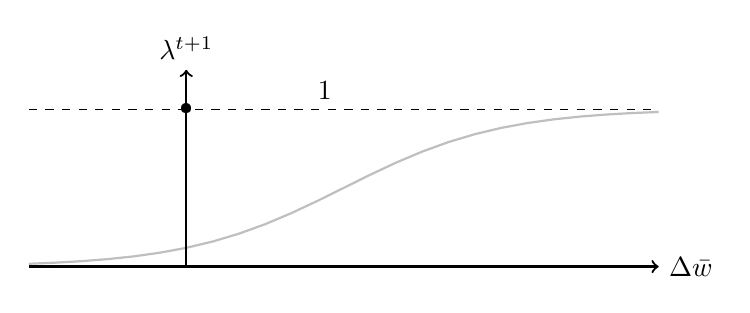
\begin{tikzpicture}
		\draw[domain=-4:4, color=lightgray, thick] plot (\x,{2/(1+exp(-\x))}); 
		\draw [thick, ->] (-4,0) -- (4,0) node [right] {$\Delta \bar{w}$};
		\draw [thick, ->] (-2,0) -- (-2,2.5) node [above] {$\lambda^{t+1}$};
		\draw [dashed] (-4,2) -- (4,2) node[pos=0.47, above] {$1$};
		\node at (-2,2) {\textbullet};
		\end{tikzpicture}
	\end{center}
	\caption{Increasing proportion of elected leaders in the population as average fitness increases as a consequence of leadership.}
	\label{fig:lambda}
\end{figure} 

\section{Resources production}
\label{sec:prod}

Every individual possesses the same time budget, which constrains a trade-off between individual production and group action. One invests a proportion $\tau_i$ of their total time budget into production, that is, extraction of natural resources. Productivity at the population level corresponds to the extraction rate of natural resources, which increases as a function of technology $\nabla$ available at time t. This available technology is cumulative and results from the previous generations' public good resources dedicated to innovations for productivity enhancement. The amount of extracted resources, or productivity, depends on the extraction rate $\beta$ pertaining to the society's technological means. Thus, $\beta$ follows a law of diminishing marginal returns as a function of the aforementioned technological resources. Technology therefore governs the extraction rate of natural resources such as:

\begin{equation}
\beta = f\left(\nabla\right)
\end{equation}
 
Where $f$ is an increasing function of $\nabla$ (fig. \ref{fig:betafunc}) and $0\le\beta\le1$.

\begin{figure}[!htbp]
	\begin{center}
		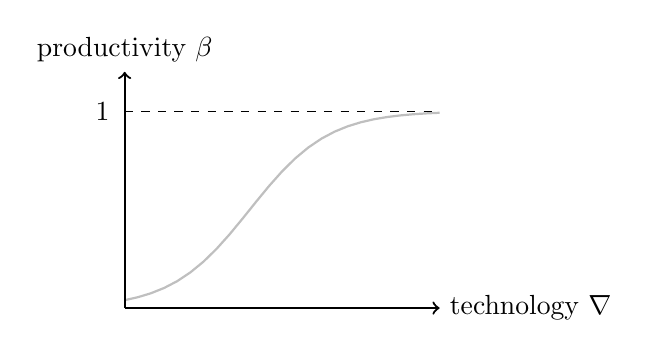
\begin{tikzpicture}
		\draw[domain=0:4, color=lightgray, thick] plot (\x,{2.5*0.1*exp(2*\x)/(2.5+0.1*(exp(2*\x)-1))}); 
		\draw [thick, ->] (0,0) -- (4,0) node [right] {technology $\nabla$};
		\draw [thick, ->] (0,0) -- (0,3) node [above] {productivity $\beta$};
		\draw [dashed] (0,2.5) -- (4,2.5) node[pos=-0.07] {$1$};
		\end{tikzpicture}
	\end{center}
	\caption{Diminishing returns of extraction rate with increasing technology.}
	\label{fig:betafunc}
\end{figure} 

Let the natural resources available for extraction within the population's territory $\Omega$ be very large \footnote{Here, $\Omega$ is assumed to be fixed, but see Motesharrei et al. 2014 for possible later dynamic implementations.}, and the per-capita amount of resources obtained after extraction:

\begin{equation} \label{eq:resources}
	R_i = \tau_i\cdot\frac{\beta\left(\nabla\right)\cdot\Omega}{N}
\end{equation}

\section{Collective action}
\label{sec:collact}

Individuals in the population all participate to the maintenance of an institution, whose role is to apply collective actions in relation to productivity maximization. Two distinct cultural traits $x$ and $y$ borne by every individual in the population respectively determine (i) degree of involvement into the institution and (ii) personal preferences as for public good resources management.     

Involvement into the collective action incur individual costs in terms of resources and time. $x$ measures to proportion of own resources that one invests into the institution. The sum of all investments across the population amounts to the public good $P$. 

\begin{equation} \label{eq:pubgood}
P = \sum_{i=1}^{N}x_i\cdot R_i
\end{equation}

$P$ can be used for different purposes: increasing the level of acquired technology from the previous generations $\nabla_{t-1}$ through innovations enhancing extraction rate of natural resources; detecting and sanctioning cheaters. Cheaters are individuals in the social group who benefit from the enhanced productivity at the population level thanks to the investment into innovations from previous generations, but do not invest as much of their own resources into the current generation's public good as their peers do. Cheaters are therefore defined according to the current's generation distribution of $x$ values: they are the individuals who invest less than a predefined quartile of $X$ distribution in the population \footnote{Should $q$ \textit{i.e.} level of tolerance to cheaters / quartile change over time e.g. $25\%\to15\%$?}. Hence, I can write the proportion $\delta$ of honest individuals in the population as:

\begin{equation} \label{eq:cheat}
\delta=1-p(x\le Q_q\left(X\right))
\end{equation}

Individuals express a personal preference for the repartition of public good resources into innovations on one hand and cheaters detection and sanctioning on the other hand. This preference is defined as the proportion $y$ of the public good an individual would like to see allocated for the detection and sanction of cheaters. After deliberation, I assume that a consensus is reached over the actual proportion $h$ of public good dedicated to the detection and sanctioning of cheaters \footnote{Is there always a consensus reached or can the collective action fail overall due to too large differences in individual preferences? c.f. Simon's paper on leadership.}. The proportion of time $\chi$ required to reach a consensus is a cost incurred equally to every individual in the population, as the proportion of time $\tau$ one can allocate to personal production of resources $R_i$ is: 

\begin{equation}
\tau=1-\chi
\end{equation}

I formalize $\chi$ as a function of the population size $N$, the variance of personal preferences in the population $\sigma_Y$ and the number of leaders in the population $n_L$:

\begin{equation}
\chi = \phi\left(N,\sigma_X,n_L\right)
\end{equation}  

So that $0\le\chi\le1$. $\phi$ is an increasing function of both $N$ (\textit{i.e.} the number of voices) and $\sigma_Y$ (\textit{i.e.} the breadth of opinions on public good allocation), but decreases with leadership support, such as $\frac{\partial\phi}{\partial N}$ and $\frac{\partial\phi}{\partial\sigma_Y}>0$ and $\frac{\partial\phi}{\partial n_L}<0$.

Once reached, the consensus follows an aggregation rule. For now, I use the mean individual preference in the population to calculate the effective portion of public good dedicated to detection and sanctioning of cheaters:

\begin{equation}
h=\frac{1}{N} \sum_{i=1}^{N}y_i
\end{equation}

As a consequence, the increase in technology in the next generation, determined by the amount of public good of the current generation invested in finding and establishing an innovation \footnote{innovations are relatively rare, hence we might want to use a Poisson distribution in order to formalize the probability that a new technology improving resources extraction is found.}, is as follows:

\begin{equation}
\nabla_{t+1}=\nabla_t + g\left[\left(1-h\right)P\right]
\end{equation}

Where g is a saturating function of resources invested in ``research and development''. Technology governs the extraction rate of natural resources such as described in section \ref{sec:prod}.

\begin{figure}[!htbp]
	\begin{center}
		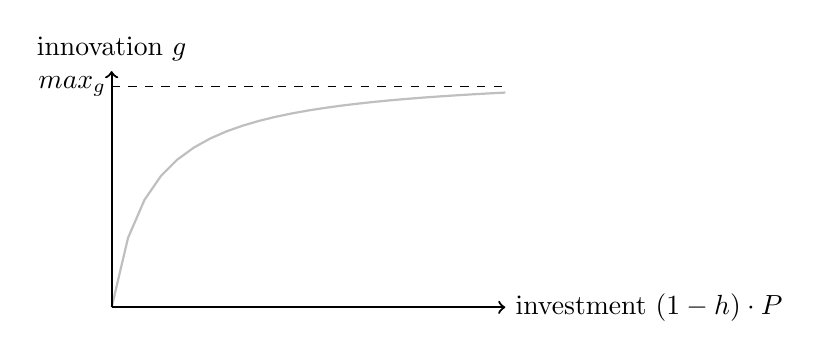
\begin{tikzpicture}
		\draw[domain=0:5, color=lightgray, thick] plot (\x,{0.6*\x/(0.1+0.2*\x)}); 
		\draw [thick, ->] (0,0) -- (5,0) node [right] {investment $(1-h)\cdot P$};
		\draw [thick, ->] (0,0) -- (0,3) node [above] {innovation $g$};
		\draw [dashed] (0,2.8) -- (5,2.8) node[pos=-0.1] {$max_g$};
		\end{tikzpicture}
	\end{center}
	\caption{Increase of technology level with investment of public good.}
	\label{fig:techfunc}
\end{figure} 

\section{Detection and punishment of cheaters}
\label{sec:cheat}

In this model, I assume that there is no false detection, meaning that the individuals detected and sanctioned are effective cheaters as defined by equation \ref{eq:cheat}. I consider that policing is a two step process, starting with the detection of cheaters followed by the sanctioning of detected cheaters. Detection efficiency is determined by the institutional quality $\kappa$, which depends on the proportion of resources specifically devoted to detection $k$ and on the population size. In other words, the institutional quality $\kappa$ is the probability for a cheater to be detected:

\begin{equation}
\kappa=\omega\left(\frac{h\cdot P\cdot k}{N}\right)
\end{equation} 

Where $\omega$ is a decreasing function of $N$ but an increasing function of $P$, with $0$ and $1$ as respective lower- and upper-bounds. I can then write the effective amount of resources devoted to active punishment of cheaters as:

\begin{equation}
F=h\cdot P\left(1-k\right)
\end{equation}

$F$ can be viewed as a fine imposed on detected cheaters by the institution. Additionally, detected cheaters are coerced into returning part of their resources to the public good. This portion corresponds to the difference between wthe porption of resources invested by the cheater and the mean portion $\bar{x}$ of resources invested by each individual in the population into the public good \footnote{For now, the average $x$ value in the population is assumed to be accurately assessed. However, one could imagine that there is a possibility of estimation error, leading to an over- or underestimation of $\bar{x}$.}. This allows me to write the payoff for each individual $i$ from each social class $j\in$ \{producer, leader\}\footnote{Ideas for producers alternatives (considering leaders can also produce, technically): plebeians, civilians, citizens} as:

\begin{equation}
\pi_{i,j}=\delta\cdot(1-x_i)\cdot R_i+\left(1-\delta\right)\left[\kappa\left(R_i\left(1-\bar{x}+x_i\right)-\frac{F}{\kappa\left(1-\delta\right)N}\right)+\left(1-\kappa\right)\cdot(1-x_i)R_i\right] 
\end{equation}

\section{Cultural transmission}
\label{sec:trans}

This model aims to explore the evolutionary dynamics of two cultural traits. The transmission modes of each trait are described in the following sections and synthesized in figure \ref{fig:cultrans}. I assume that individuals are norm followers, in that their strategies quantified by $x$ and $y$ values are both independent of their payoff \footnote{Later on, I will try to compare with a model considering that every player is rational, and then combine both norm followers and rational individuals.}. 

\subsection{Investment in institution}

$x$ is the proportion of its own resources an individual is willing to invest into institutions. This cultural trait is vertically transmitted, acquired directly from the parent $x$ value with probability $d^x$. There is a chance $1-d^x$ for social transmission not be direct, in which case the focal subject is randomly socialized by any other individual from the parental generation.

\subsection{Policing preference}

$y$ is the personal preference of an individual for the proportion of public good that should be dedicated to policing. This trait is initially vertically transmitted in a similar manner as trait $x$, with a probability $d^y$ for direct transmission and $1-d^y$ for socialization by another individual from the parental generation. However, upon reach of adulthood, individuals might be subject to social influence from peers, with elected leaders having more impact than others. Thus there is a probability $d^{\text{II}}$ that the individual is secondarily socialized by a leader or a producer, chosen semi-randomly within the population, with leaders $m$ times more likely to secondarily influence individuals through say, media for instance.  

\begin{figure}[!htbp]
	\centering
	\begin{subfigure}{.5\textwidth}
		\centering
		\captionsetup{width=.9\linewidth}
		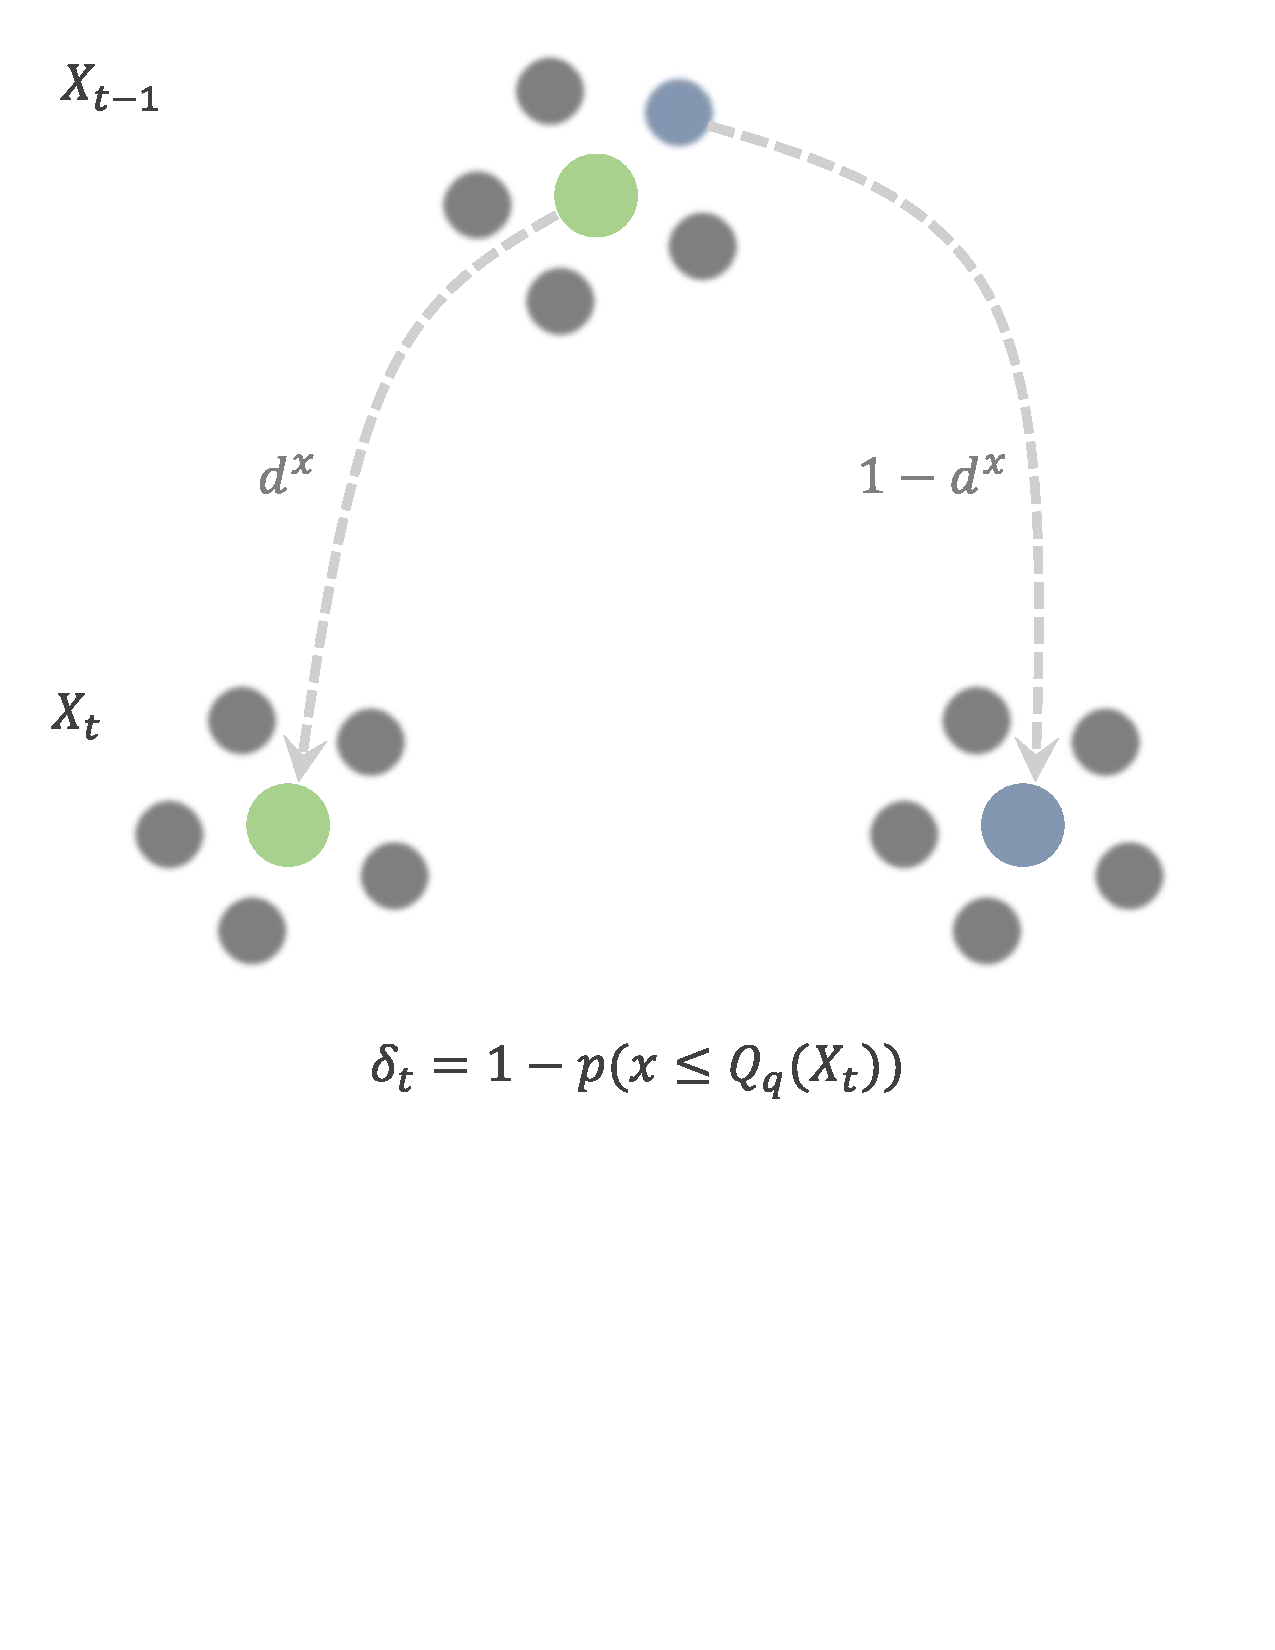
\includegraphics[width=.9\linewidth]{xTransmission.pdf}
		\caption{Vertical transmission of the cultural trait $x$, measuring the individual resources investment level in institutional.}
		\label{fig:xtrans}
	\end{subfigure}%
	\begin{subfigure}{.5\textwidth}
		\centering
		\captionsetup{width=.9\linewidth}
		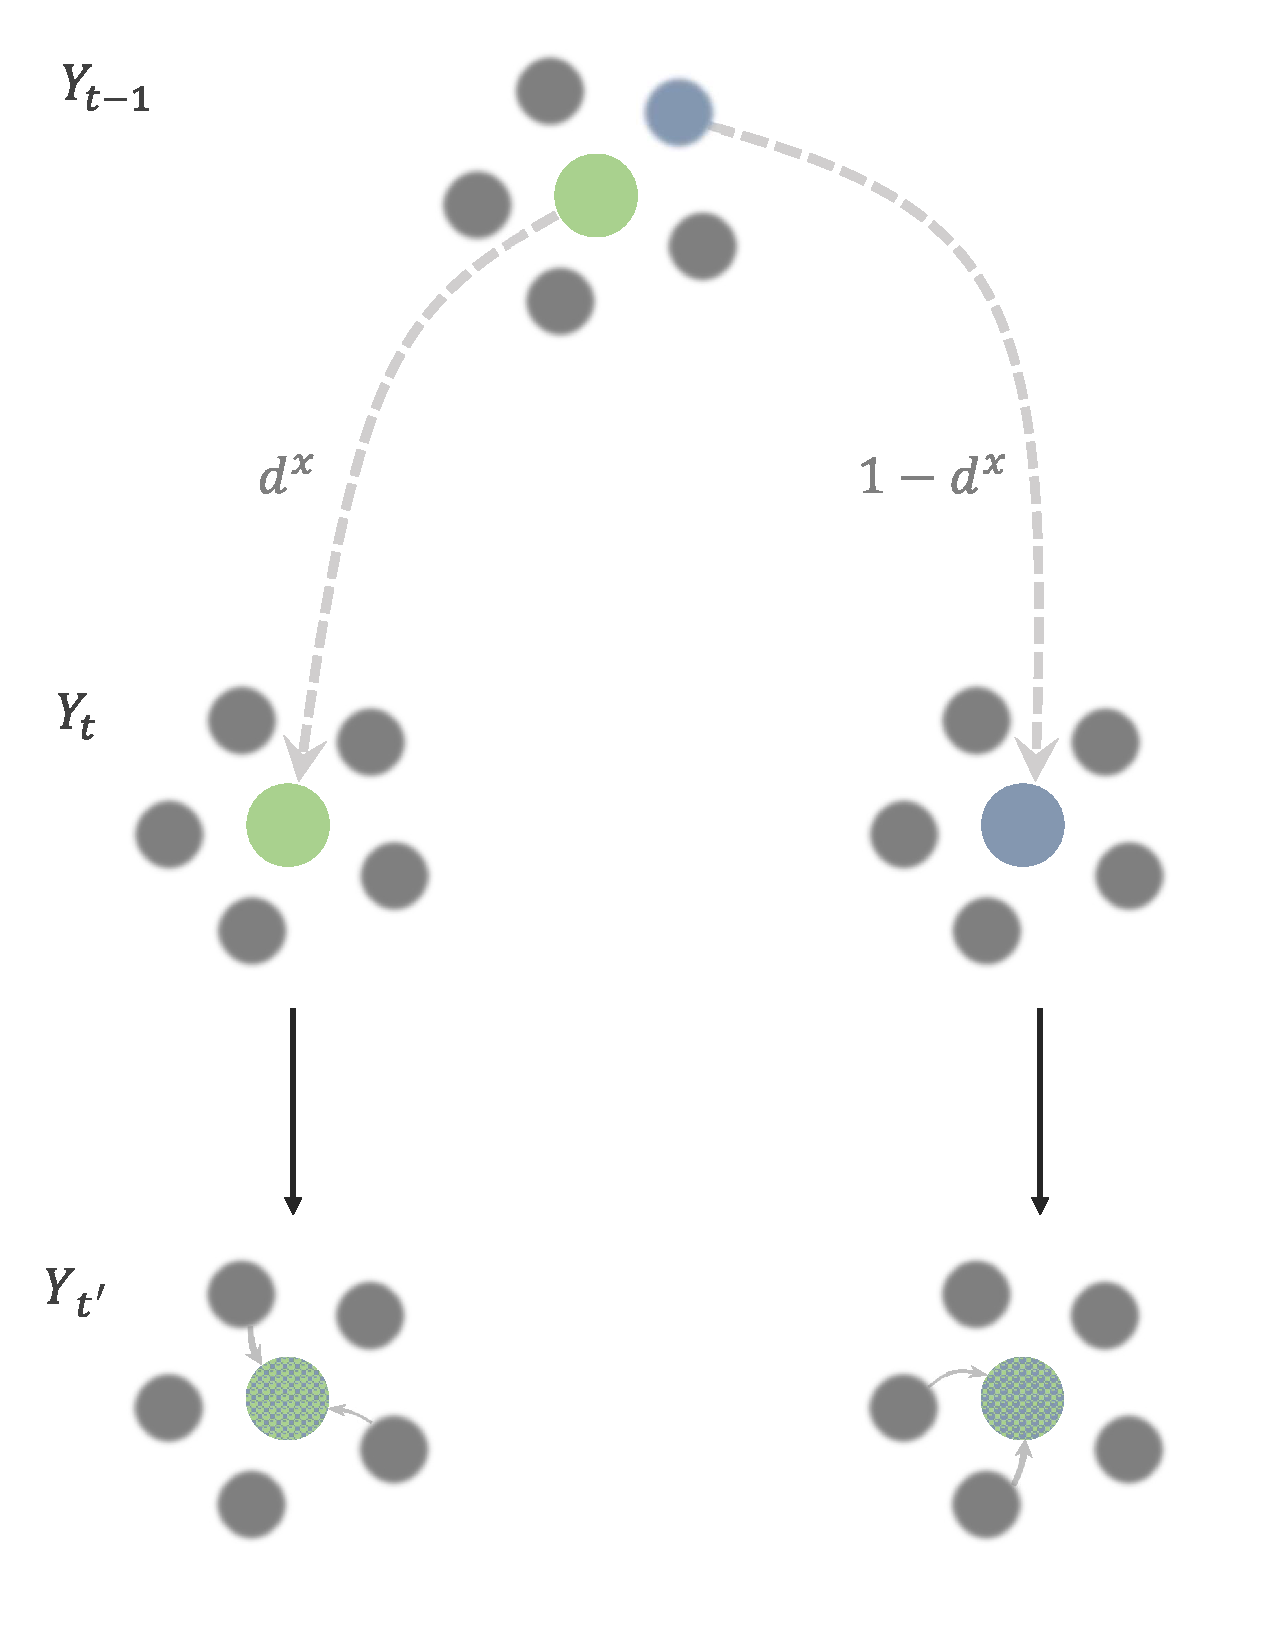
\includegraphics[width=.9\linewidth]{yTransmission.pdf}
		\caption{Transmission steps of the cultural trait $y$, measuring personal policing preference. Vertical primary transmission followed by secondary horizontal socialization, \textit{i.e.} from peers.}
		\label{fig:ytrans}
	\end{subfigure}
	\caption{Differential transmission modes of the two cultural traits studied in the model}
	\label{fig:cultrans}
\end{figure} 

\section{Reproduction}
\label{sec:repro}

Leaders are assumed to be politically trustworthy in the sense that they effectively dedicate a greater portion of their own time to solving collective action problems, in order to decrease the total time necessary to reach a consensus, and thus enable producers to dedicate more of their own time to natural resources extraction. However, I postulate that individuals have an acute sense of fairness, which implies that leaders will only take on their role if they obtain a final wealth at least equal to the final resources of non-leaders. Hence, if per-capita leader and producer income is $\rho_L$ and $\rho_P$ respectively, the condition for leaders to agree upon sacrificing more of their valuable time than others is $\rho_L\ge \rho_P$. In order to fulfill this condition and thus alleviate the extra-burden that they endure as leaders, elected individuals are entitled to levy taxes, which are formalized as the transfer of a proportion $\alpha$ of producer resources to leaders. Assuming further that leaders do not exploit producers (supposing for example that despots would be automatically exposed and overthrown by the population), I can write:

\begin{equation}
\begin{aligned}
\rho_P = \rho_L \Leftrightarrow\frac{\sum_{i=1}^{n_P}(1-\alpha)\pi_{i,P}}{n_P} &= \frac{\frac{\sum_{i=1}^{n_P}\alpha\pi_{i,P}}{n_L}+\sum_{i=1}^{n_L}\pi_{i,L}}{n_L}\\
n_L^2 \sum_{i=1}^{n_P}(1-\alpha)\pi_{i,P} &= n_P\left(\sum_{i=1}^{n_P}(\alpha\pi_{i,P}) + \sum_{i=1}^{n_L}(\pi_{i,L})\right)\\
\alpha &= \frac{n_L\left(n_L\Pi_P+n_P\Pi_L\right)}{\Pi_P\left(n_p+n_L^2\right)}
\end{aligned}
\end{equation}   

Where $\Pi_j=\sum_{i=1}^{n_j}\pi_{i,j}$. Individual final resources determine lifetime reproductive success $W_{i,j}$. I assume that collected taxes are equally shared between leaders. There is intra-class competition for resources, characterized by the terms $\gamma_L$ and $\gamma_R$.

\begin{equation}
\begin{cases}
w_{i,L}=\frac{r_L+\pi_{i,L}+\frac{\alpha\Pi_P}{n_L}}{1+\gamma_L n_L}\\
w_{i,P}=\frac{r_P+(1-\alpha)\pi_{i,P}}{1+\gamma_P n_P}
\end{cases}
\end{equation}

Where $r_L$ and $r_P$ correspond to the basic resources an individual should have access to each class, in absence of intra-class competition ($\gamma_j=0$).

\section{Base average fitness}

The base average fitness at generation $t$, $\bar{w}_0$, is an information accessible to the next generation $t+1$. It corresponds to an estimate of the fitness of individuals at generation $t$, calculated over the whole population, were the social group to be acephalous at this period of time, \textit{i.e.} $\lambda_t=n_L^t=0$. The crucial variable in calculating $\bar{w}_0$ is $\chi$. As I want to know the effect of leadership absence on average fitness, I can write:

\begin{equation}
	\chi_0=\phi(N^t,\sigma_{X_t},0)
\end{equation}

From this, the complete dynamic of acephalous collective action can be deduced, and $\bar{w}_0$ estimated. I then have:

\begin{equation}
	\Delta\bar{w}=\frac{w_{i,L}\cdot n_L+w_{i,P}\cdot n_P}{2}-\bar{w}_0
\end{equation}
%\bibliographystyle{plain}
%\bibliography{bibliography.bib}
\end{document}